% Chapter Template

\chapter{The Mesh Architecture} % Main chapter title

\label{Chapter2} % Change X to a consecutive number; for referencing this chapter elsewhere, use \ref{ChapterX}

\lhead{Chapter 2. \emph{The Mesh}} % Change X to a consecutive number; this is for the header on each page - perhaps a shortened title

In this chapter, we will look at the short range communication architecture for inter communication among the UAVs which entails realizing a wifi mesh network based on the IEEE standard 802.11s. We shall also look at how it is integrated into ROS.

%----------------------------------------------------------------------------------------
%	SECTION 1
%----------------------------------------------------------------------------------------

\section{IEEE 802.11s}
The IEEE WLAN 802.11 standard is quite a popular solution for high bandwidth networking services at reasonable distances. But, it is based on a centrailized architecture, where every networking node is a \textit{Station}, STA. In the simplest architecture, one of the STAs acts as an \textit{Access point}, AP, a centralized node which provides integration services to other STAs. It is a single hop architecture where \textit{STAs} directly communicate with \textit{APs}, and all the communication between \textit{STAs} is routed through the \textit{AP} to which they are connected. Essentially, it is a network in star configuration, at MAC layer.

With growing demand for more diverse wireless infrastructure and multihop networks, 802.11s \cite{802.11s} emerged as an ammendment to the original standard to accommodate mesh networking architecture. The 802.11s standard extends the 802.11 MAC layer, allowing a MAC based multihop architecture.

\begin{figure}
	\centering
	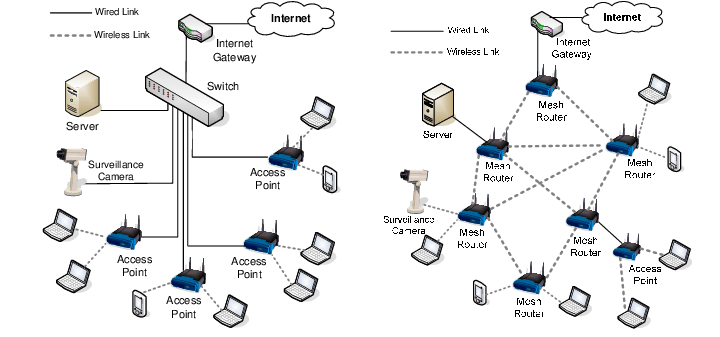
\includegraphics[scale=0.6]{Pictures/80211s.png}
	\caption{A comparison of 802.11 wlan and 802.11s mesh networks}
	\label{fig: 80211s}
	\captionsetup{font={footnotesize,bf,it}}
	\caption*{source: Portmann, Marius. (2006). Wireless Mesh Networks for Public Safety and Disaster Recovery Applications. 10.1201/9781420013542.ch16. }
\end{figure}

\subsection{Routing in 802.11s}
Though there are a lot of routing protocols proposed in wireless mesh networks, the field is still active in research. What routing protocol to use closely depends on the application, and choice of the routing protocol may significantly impact the performance of the system.  